95. $\cfrac{(-1+x^2)(x+1)^2(x-1)^3}{x^8-x^6+x^4}\leqslant0\Leftrightarrow\cfrac{(x-1)^4(x+1)^3}{x^4(x^4-x^2+1)}\leqslant0.$ Применив метод интервалов, найдём ответ: $x\in(-\infty;-1]\cup\{1\}.$
\begin{figure}[ht!]
\center{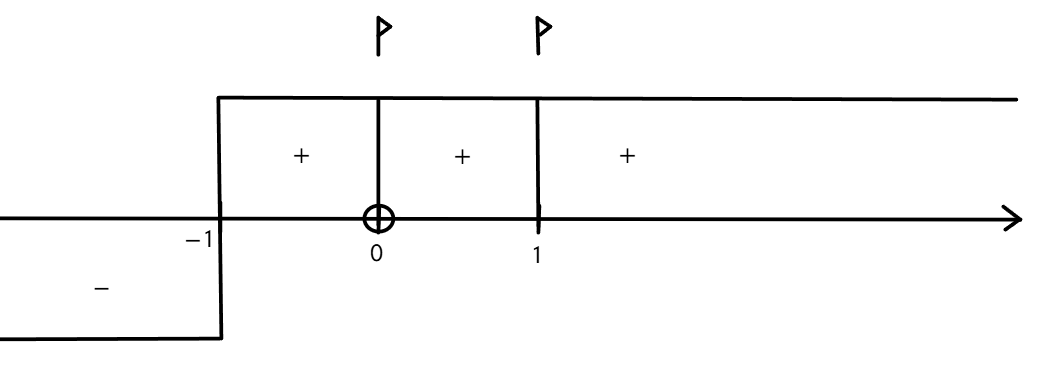
\includegraphics[scale=0.35]{ner99-33.png}}
\end{figure}

ewpage
